%*****************************************
\chapter{Introduction}
\label{chapter:chapter intro}
%*****************************************

\section{ Social Network Analysis in health }

In recent years there has been a growing recognition of the profound impact that social relationships and networks of friends have on health outcomes (figure \ref{figure:networkNetworkRise}). This includes common and well-known topics such as the spread of obesity \cite{Christakis2007, Trogdon2008}, recreational drugs usage such as smoking \cite{Christakis2008, Aschbrenner2018} alcohol \cite{Rosenquist2010, Ali2014} or cannabis \cite{Mednick2010}, and  depression \cite{Rosenquist2010}.

    \begin{figure}[H]
        \centering
            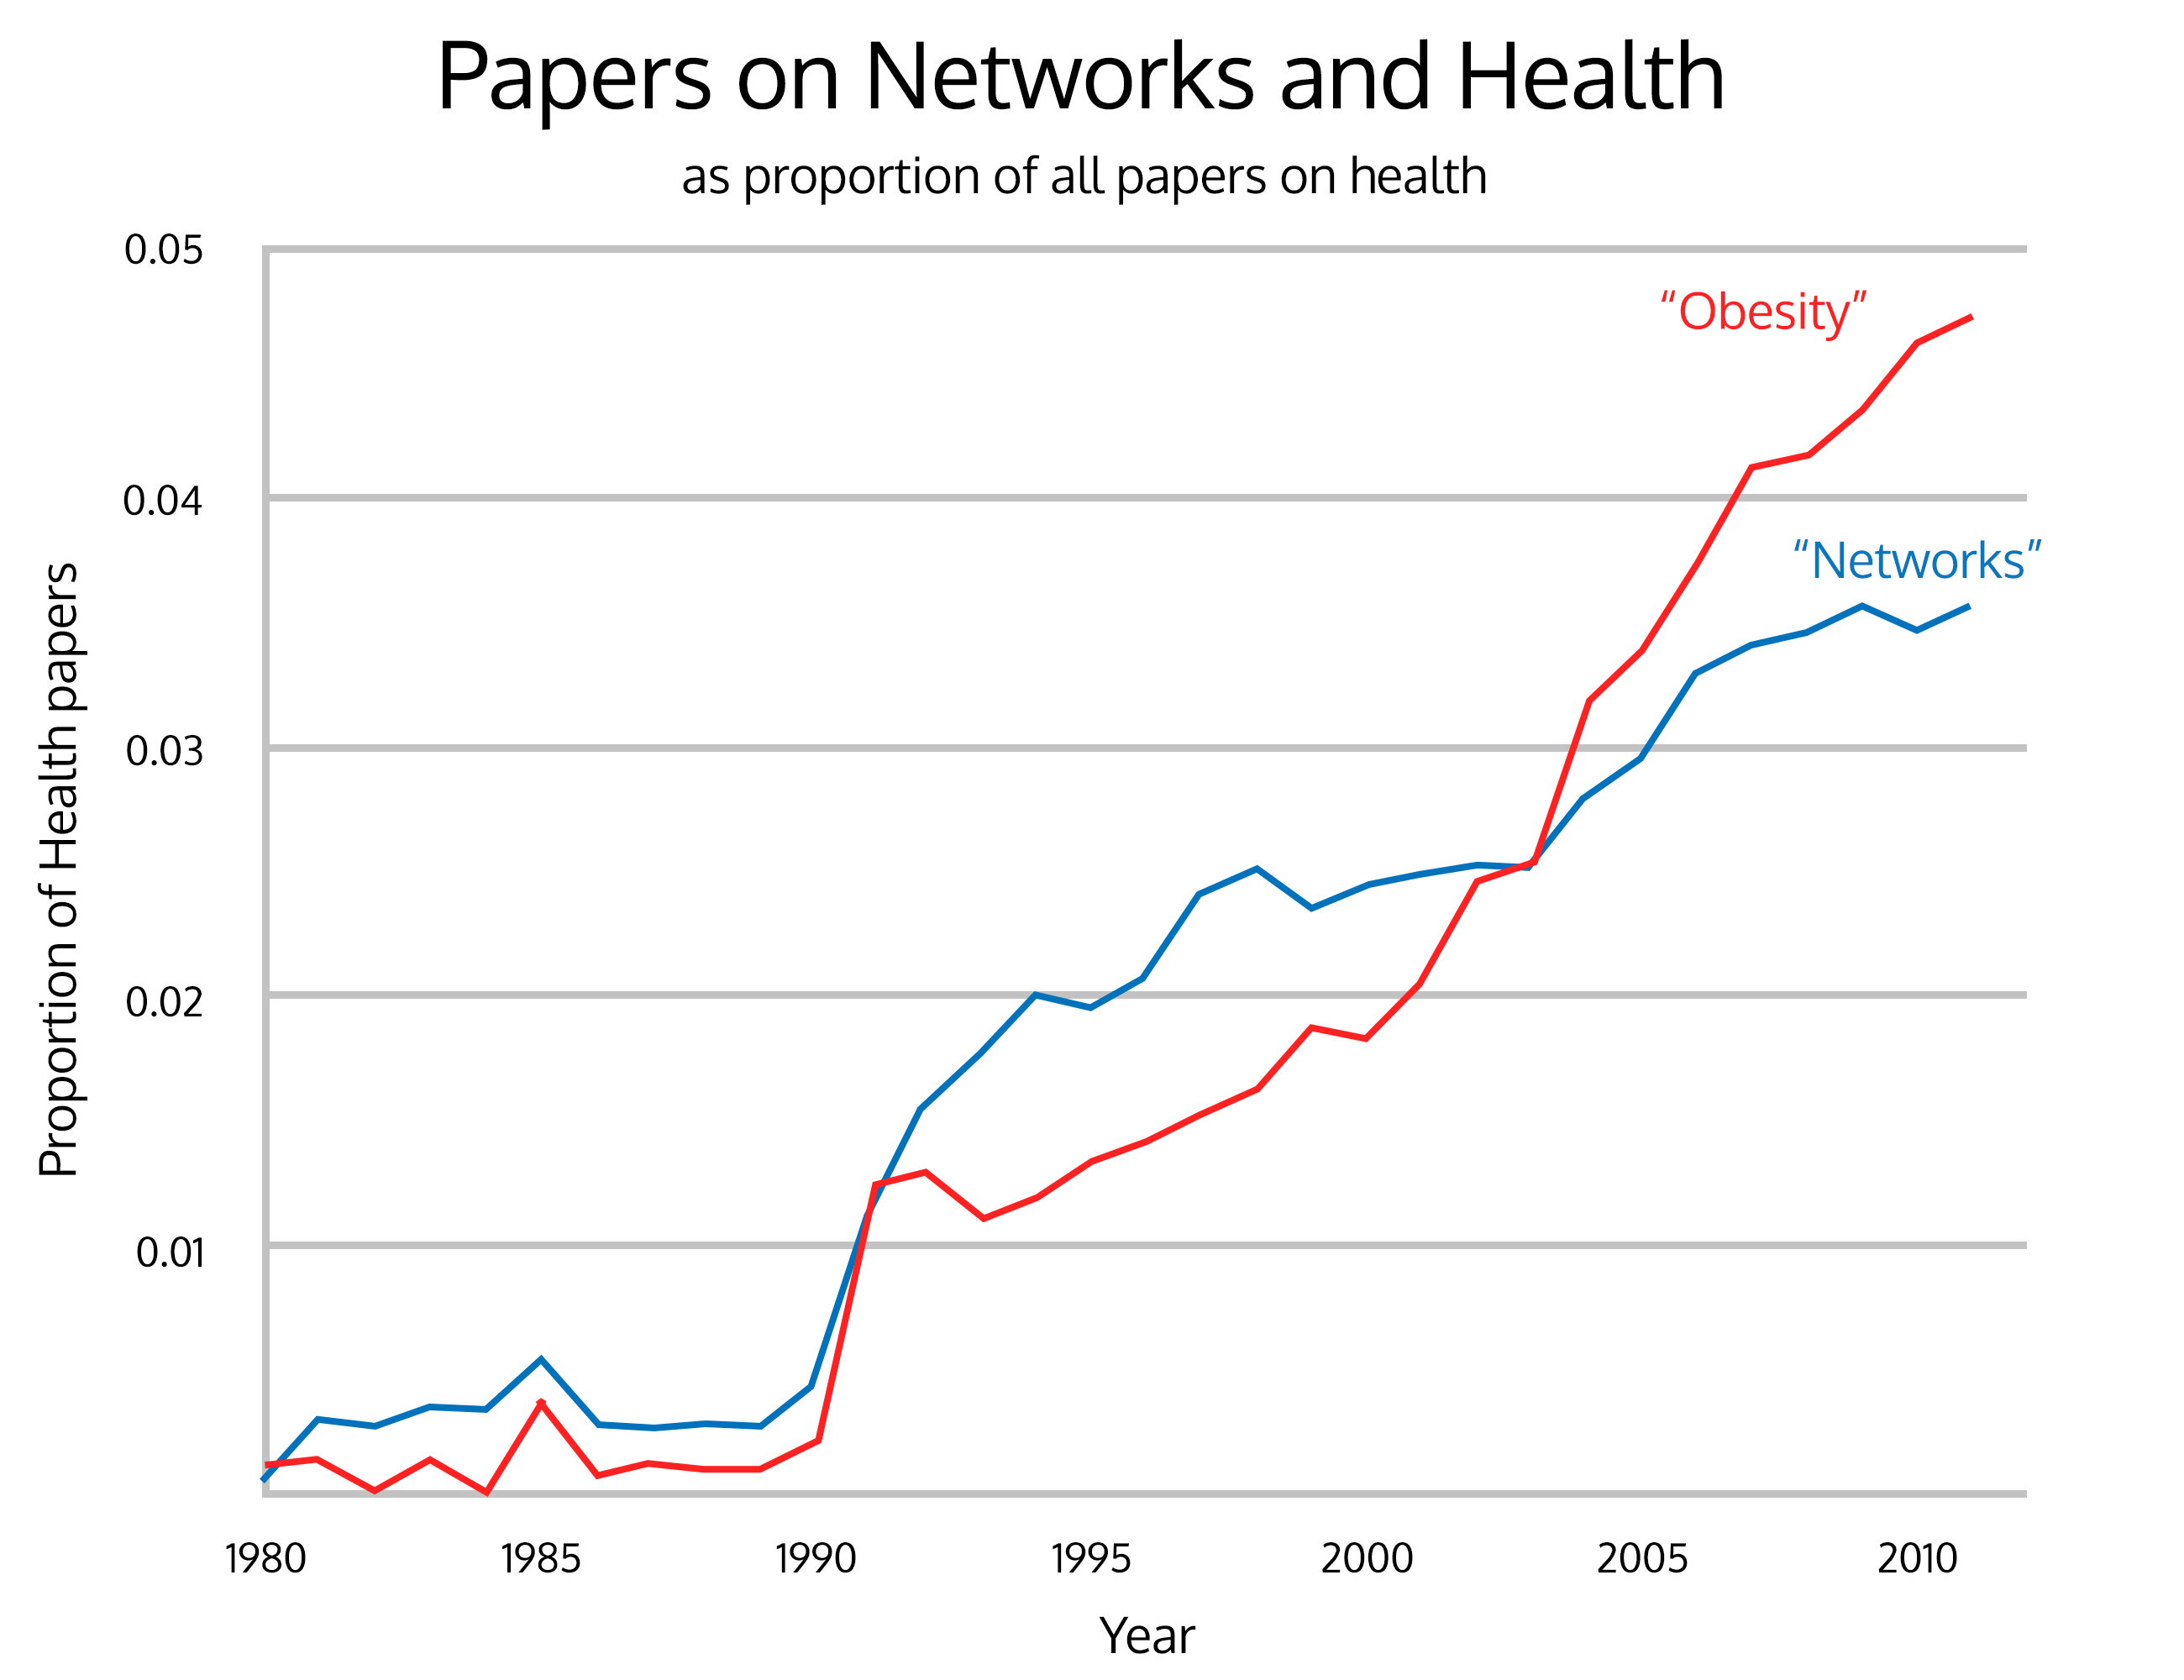
\includegraphics[width=0.7\linewidth]{figures/Social/paperSocialRemastered.png} 
        \caption{Proportion of papers published about networks on the topic of health across the years, compared with the number of papers published on obesity. Image reproduced with permissions from "International Encyclopedia of the Social and Behavioral Sciences" \cite{ref:networkRises}.}
        \label{figure:networkNetworkRise}
    \end{figure}

\gls{sna} is a powerful tool for understanding how social connections influence health behaviors, disease transmission, and healthcare access. This thesis leverages \gls{sna} techniques to explore the dynamic interplay between social networks and health, aiming to provide valuable insights that can inform interventions, policies, and practices for improving health outcomes.

\section{ Social network interventions }
\label{socialinterventions}

Within the realm of health research, \gls{sna} has demonstrated its versatility and applicability across a wide range of topics. It is possible to detect early outbreaks of influenza \cite{Christakis2010}. To prevent the spread of \gls{hiv} infections \cite{Friedman1997}. To improve the life of chronic illnesses patients as well as their families and community \cite{FernndezPea2020}. It has been shown that information on social networks can increase the prediction of health-related models at around 50\% \cite{Lin2019}. It has been used to design interventions and strategies to enhance communication, collaboration, and knowledge sharing among health professionals, ultimately improving the overall performance and effectiveness of the health organization \cite{Tasselli2014, Sabot2017}. A systematic review of 37 studies suggests that social network interventions are associated with positive health behaviors and outcomes \cite{Hunter2019}. And of course, social network interventions have been used to better the outcome of obesity \cite{Gesell2013, systems9030066, Smith2020, McGlashan2019}, mental health \cite{Pinto2005, Rosychuk2009}, overcoming tobacco addiction \cite{Latkin2015, Sadasivam2016},  transmittable diseases in humans \cite{Danon2012, Wang2011, Llupi2016, Ljubic2019} and in cattle such as cows, sheep, and pigs \cite{Marquetoux2016, OrtizPelaez2006}, and recently we experienced these interventions first hand with COVID-19 \cite{Corcoran2022, Centola2020}.

These few examples show that \gls{sna} has proven practical value in understanding the diffusion of diseases, as well as tracking the spread of infectious agents through clusters or interconnected social groups. It has been found to play a crucial role in improving individuals' health and preventing further deterioration of their well-being. Different authors have evaluated that social relationships influence a person's health between 15\% to 40\% \cite{ref:socialinfluence2014}, putting it ahead of the environment and even medical care. And yet it remains a vastly under-utilized and underrated technique.

\section{ Thesis impact }

In this thesis, we employ \gls{sna} techniques to shed light on the complex relationships between social networks and health outcomes within a specific population. We have shown how \gls{staph}, vitamin D, inflammation, medication usage, and obesity are influenced by social networks in a general youth population in Tromsø. We also expanded non-parametric methods for group comparisons in graphs using simulations and applied machine learning models to measure the influence of peers on obesity. Finally, we lay down the basics for a framework to obtain a more efficient analysis framework. We hope this leads to a significant contribution to public interventions and policies that ultimately lead to improved health outcomes in Norway and beyond.
